Before we can discuss subtracting the $4\pi$ background, we need to deal with another source of background which we cannot avoid with cuts. As mentioned in \Cref{subsub:combos}, each event in the dataset holds multiple ``combos''\textemdash alternate hypotheses for the set or ordering of the particles which make up the topology. For example, in the $K_S^0K_S^0$ final state, there are two identical $\pi^+$ and $\pi^-$ particles. The choice of which $\pi^+$ goes with which $\pi^-$ to form each kaon is partially constrained by th kinematic fit, but in the case where both pion combinations yield results which pass through the entire reconstruction and particle identification process, both are included as separate combos in the same event. The fiducial selections we performed in \Cref{sub:fiducial-cuts} eliminate many of these combos, since the incorrect combinations will sometimes have very high $\chi^2_\nu$, but there may be some remaining at the end of these selections. For this combinatoric case, we can reduce the effect of incorrect combinations by only selecting the combo with the lowest $\chi^2_\nu$ in each event. While this does not guarantee that we will have the correct combination, it will prevent us from double-counting, and it is more likely that the best $\chi^2_\nu$ is the true event.

Additionally, we can get combos from different beam photon combinations. If multiple tagged photons have energies which are compatible with the reaction, each is included as a separate combo. It can also be the case that the true photon was simply not reconstructed, and some incorrect photon which was close enough was matched with the combo instead. In either case, we have multiple combos which do not correspond to their true beam events. We call both of these cases ``accidental'' combos. To account for this, we first recall that the accelerator produces beam bunches every $\SI{4}{\nano\second}$ in radio-frequency (RF) bunches. A beam bunch consistent with a given event is labeled ``in-time'', while the surrounding bunches are called ``out-of-time''. We can reduce the impact of these accidental combos by estimating the contribution they have on the in-time events and using out-of-time events as a negatively-weighted background estimation. Since the in-time accidentals are indistinguishable from true events, we must use events which also pass through kinematic selections in our subtraction, and these out-of-time events are kinematically good events. The estimation of the scaling for these out-of-time contributions has been calculated via systematic studies of the various tagger components. For our data, we choose to include eight bunches of accidentals, although we cut out the nearest bunches to avoid using in-time events in our subtraction. The distribution of the difference in RF times with respect to the event time is shown in \Cref{fig:delta-t-rf}. In this figure, the in-time events are located in the peak centered at zero, and we cut the peaks immediately on either side, and we define the boundaries between peaks using a peak width of $\SI{4}{\nano\second}$\footnote{The exact value used is $\SI{4.008016032}{\nano\second}$.}. The remaining three out-of-time peaks on either side are given a negative weight (approximately $1/6$th for each) while the in-time peak gets a weight of $1$.

To unify this accidental subtraction with the combinatoric reduction done by selecting the best $\chi^2_\nu$, we first perform the $\chi^2_\nu$ selection, which will reduce each event to a single combo (some of which might be in the out-of-time peaks), and then we carry out the accidental subtraction. At this stage, the only background which remains unaccounted for is that of incorrect topologies disguised as our signal.

\begin{figure}
  \begin{center}
    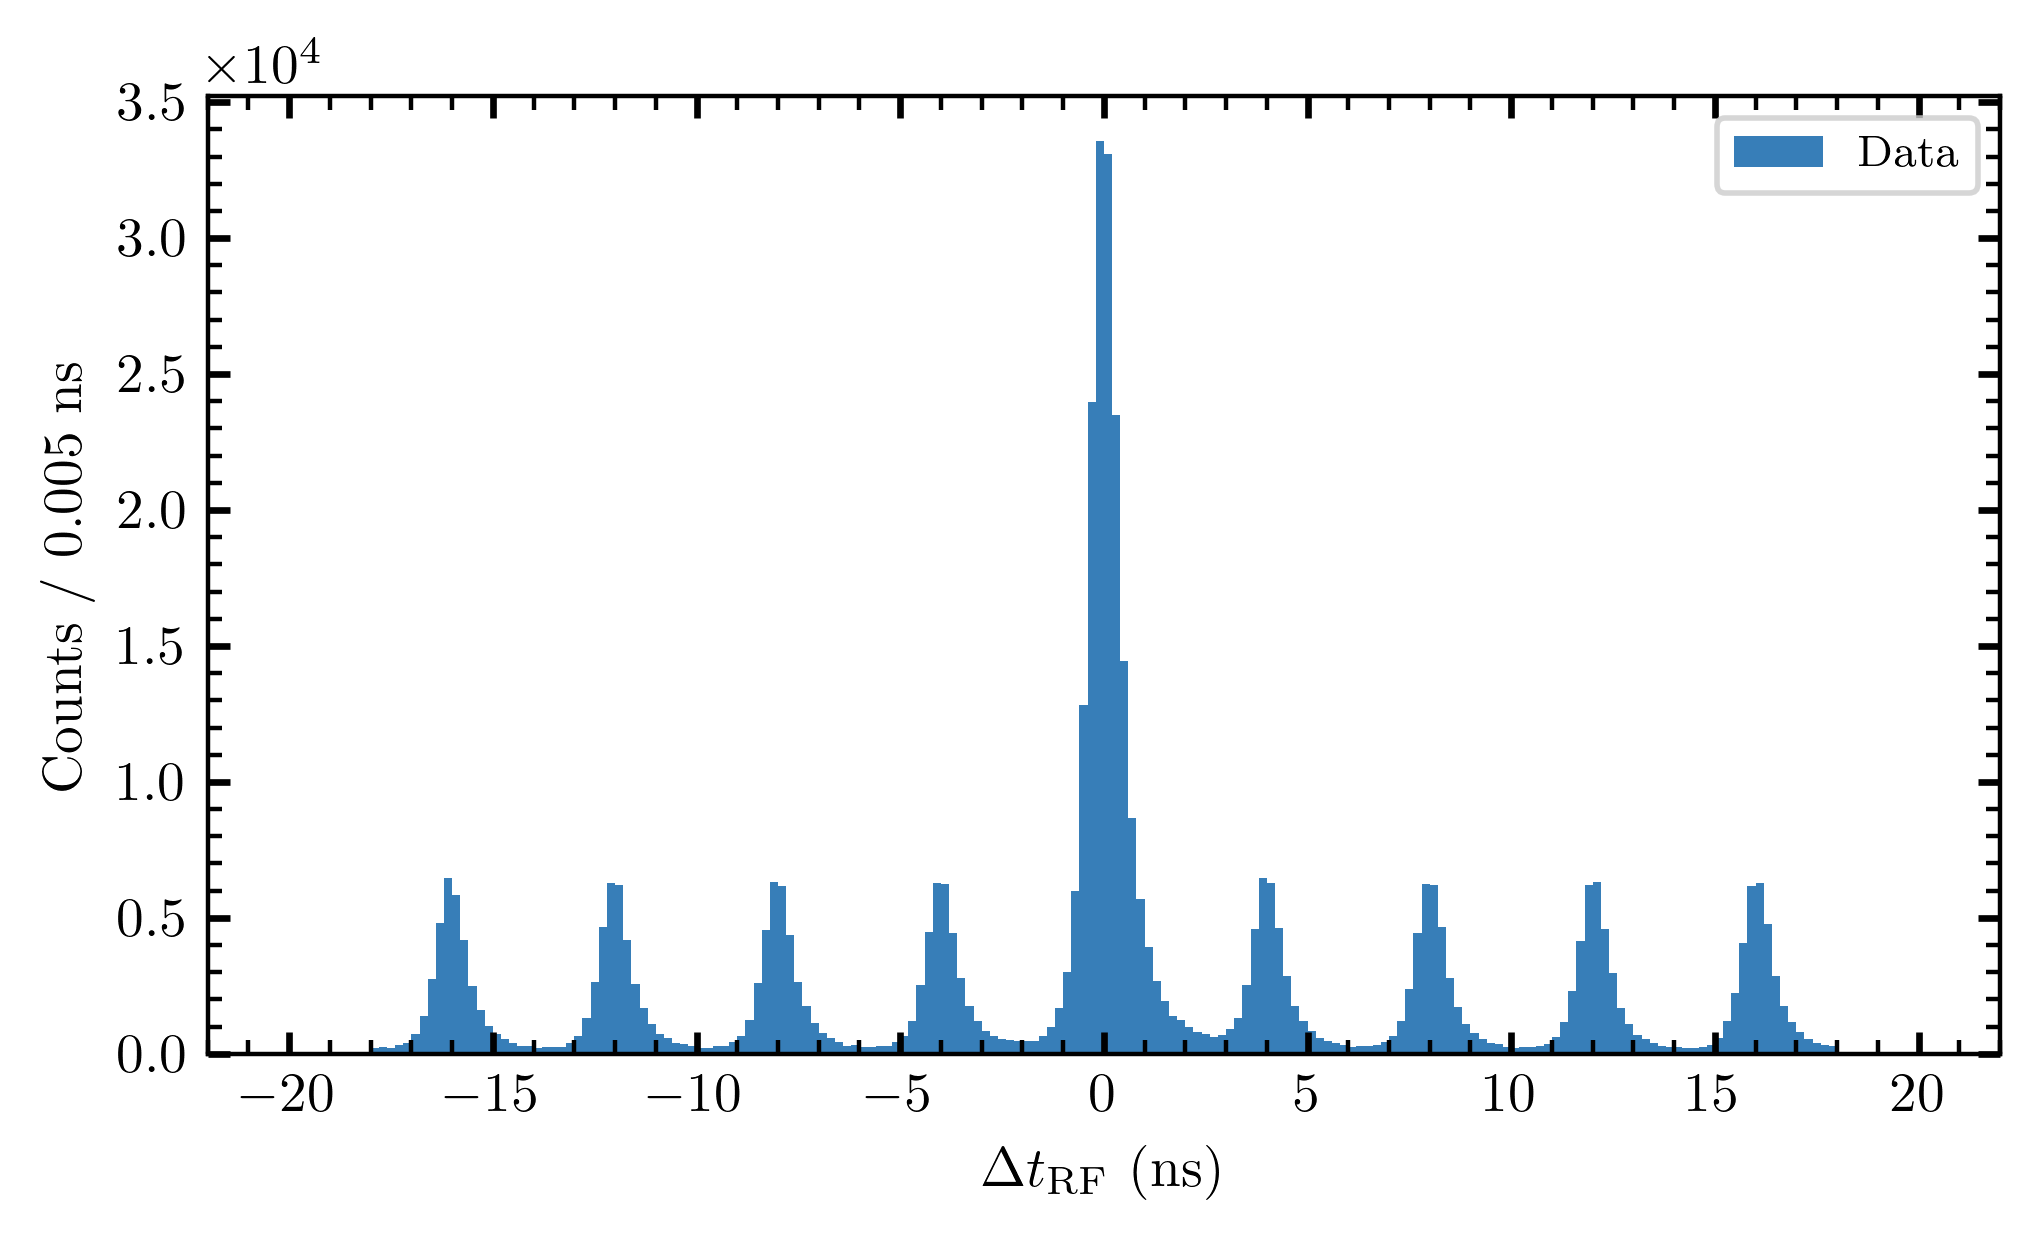
\includegraphics[width=0.8\textwidth]{figures/data_original_RF_chisqdof_3.4_protonz.png}
  \end{center}
  \caption{The time difference between the RF time recorded by the tagger and the event time. The main peak in the middle contains in-time events while the four peaks on either side are the out-of-time events added to the dataset to simulate accidental combos in the main peak.}\label{fig:delta-t-rf}
\end{figure}
